\section{L01-Introduzione}
\subsection{Introduzione}
La \textbf{termodinamica} è la scienza che studia \textbf{l’energia}, la \textbf{materia} e le \textbf{leggi} che governano le loro interazioni (scambi).
\subsubsection{Sistema termodinamico}
Il sistema termodinamico è inteso come porzione di spazio limitata da un \textbf{contorno} che lo racchiude completamente (il contorno è costituito da una superficie reale o immaginaria, rigida o deformabile).\newline
\newline
Tutto ciò che è esterno al sistema termodinamico è il \textbf{mondo esterno} e quando il mondo esterno è di massa infinita viene chiamato \textbf{ambiente}.\newline
\newline
I termini \textbf{serbatoio}, \textbf{sorgente} o \textbf{pozzo} fanno riferimento ad ambienti che interagiscono con il sistema termodinamico.\newline
\newline
Un \textbf{sistema composto} è un insieme di sistemi e sottosistemi a massa finita e/o infinita.\newline
\newline
Il sistema può essere \textbf{monocomponente} (sostanza pura o miscela di sostanze pure in rapporto fisso, quale ad esempio l'aria) o \textbf{policomponente} cioè composto da più componenti.\newline
\newline
Ogni sistema monocomponente può essere in diversi \textbf{stati di aggregazione} (solido, liquido, aeriforme). I sistemi saranno \textbf{monofase} o \textbf{polifase}.
\subsubsection{Il sistema semplice}
\begin{itemize}
    \item Chimicamente e fisicamente omogeneo ed isotropo;
    \item non soggetto a campi gravitazionali, elettrici o magnetici;
    \item chimicamente inerte
    \item esente da effetti di superficie per via delle grandi dimensioni.
\end{itemize}
\subsection{Stato di equilibrio}
Lo \textbf{stato di equilibrio} è il particolare stato cui perviene spontaneamente il sistema isolato.\newline
\newline
E' \textbf{ripoducibile} e \textbf{descrivibile} da poche proprietà del sistema stesso.
\subsubsection{Variabili termodinamiche}
Il sistema all’equilibrio è compiutamente descritto attraverso un numero ristretto di \textbf{variabili termodinamiche} (anche dette grandezze o proprietà di stato, variabili o funzioni di stato).\newline
\newline
Le grandezze si dividono in:
\begin{itemize}
    \item \textbf{Grandezza intensiva}: valore \textbf{non dipende} dall'estensione del sistema (per esempio temperatura, pressione, densità). Ne
    consegue che lo stato interno del corpo non dipende dalla sua estensione.
    \item \textbf{Grandezza estensiva}: valore \textbf{dipende} dall'estensione del sistema (per esempio massa, volume). La grandezza
    estensiva è additiva e di conseguenza il suo valore riferito ad un sistema
    risulta somma dei valori relativi ai sottosistemi che lo compongono.
    \item \textbf{Grandezza estensiva specifica}: grandezza estensiva divisa per un'altra grandezza estensiva (tipicamente massa o numero di moli, per esempio $v = \frac{V}{M}$).
\end{itemize}
\begin{center}
    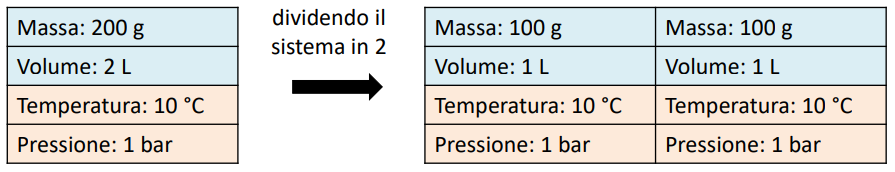
\includegraphics[height=2cm]{../L01/img1.PNG}
\end{center}
Le grandezze estensive specifiche ed intensive vengono normalmente usate per descrivere lo stato di equilibrio di un sistema termodinamico.\newline
\newline
Indicheremo le grandezze estensive, riferite cioè all'intera massa, con le lettere maiuscole e le estensive specifiche con le lettere minuscole.\newline
\newline
\textbf{Leggedi Duhem}:\newline
«Nel caso di sistema monocomponente, il numero di parametri termodinamici intensivi o estensivi specifici indipendenti atti a descrivere compiutamente lo stato interno di equilibrio è due.»
\subsubsection{Regola di Gibbs}
La differenza di ruolo tra grandezza estensiva specifica ed intensiva è messa in evidenza dalla regola di Gibbs
\[
    V = C+2-F
\]
$C$: numero di componenti;\newline
$F$: numero di fasi;\newline
$V$: numero di variabili intensive indipendenti utilizzabili.\newline
\newline
Concludendo la coppia intensiva-intensiva è sufficiente a descrivere il sistema monocomponente monofase, mentre per il sistema monocomponente bifase sarà necessaria la coppia intensiva-estensiva e per il sistema monocomponente trifase sarà necessaria una coppia estensiva-estensiva. 
\subsection{Tipologie di sistemi termodinamici}
Tipologie di \textbf{contorni}:
\begin{center}
    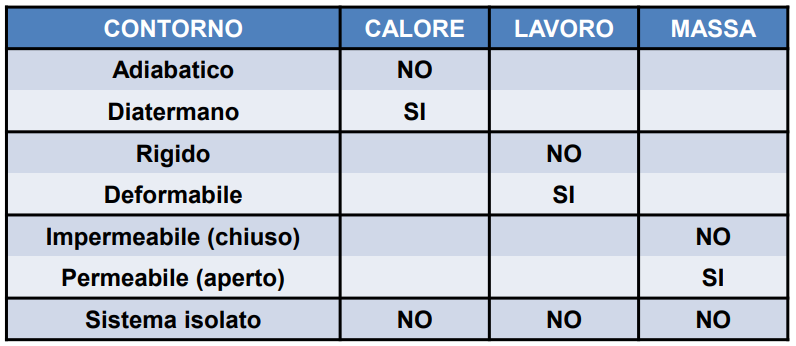
\includegraphics[height=4cm]{../L01/img2.PNG}
\end{center}
Sistema \textbf{aperto} e \textbf{chiuso}:\newline
Si parlerà di sistema chiuso se il contorno del sistema non consente scambi di massa con l’esterno; in tal caso la massa del sistema rimane costante mentre sono possibili scambi di energia sotto forma di lavoro e/o di calore con l’ambiente circostante. Un caso particolare di sistema chiuso è costituito dal sistema isolato il quale non ha scambi di energia con l’esterno.\newline
Il sistema viene inoltre definito aperto se può scambiare con l'ambiente massa.
\begin{center}
    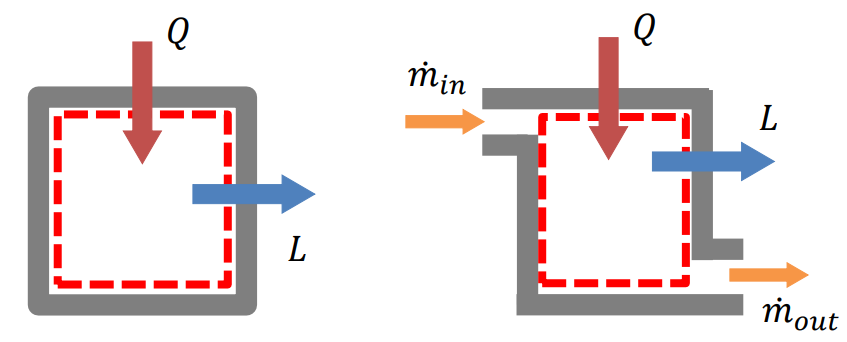
\includegraphics[height=3cm]{../L01/img3.PNG}
\end{center}
\subsection{Trasformazioni termodinamiche}
L’\textbf{insieme degli stati intermedi} successivi, tra lo stato iniziale e finale, a seguito di una variazione del sistema termodinamico, definisce la \textbf{trasformazione termodinamica}.\newline
\newline
Le trasformazioni termodinamiche si dividono in:
\begin{itemize}
    \item \textbf{Quasi-statica} o \textbf{internamente reversibile}: Costituita da una successione di stati di equilibrio; può non essere reversibile. 
    \item \textbf{Reversibile}: Se percorsa in senso inverso, riporta il sistema e ambiente nello stasto iniziale. Per trasformazione reversibile si intende spesso una trasformazione lenta.
    \begin{itemize}
        \item Traformazione \textbf{internamente reversibile}: nessuna irreversibilità si verifica all'interno del sistema.
        \item Trasformazione \textbf{esternamente reversibile}: nessuna irreversibilità si verifica all'esterno del sistema.
        \item Trasformazione \textbf{totalmente reversibile (o reversibile)}: non implica alcuna irreversibilità sia all'interno sia all'esterno del sistema.
    \end{itemize}
    \item \textbf{Irreversibile}: Trasformazione in parte o per intero non reversibile. Non è rappresentabile su un diagramma di stato. Per trasformazione irreversibile si intende spesso una trasformazione veloce.
    \item \textbf{Chiusa} o \textbf{ciclica}: Gli estremi della trasformazione coicidono.
    \item \textbf{Elementare}: Se una delle grandezze di stato si manitiene costatne durante la traformazione.
\end{itemize}
\subsection{Equazione di stato nelle coordinate P,v,T}
\textbf{equazione di sato}:
\[
    f(P,v,T) = 0
\]
In molti casi, l'equazione di stato è ignota.\newline
\newline
L’ \textbf{equazione di stato} di un \textbf{sistema semplice} è rappresentata in uno spazio cartesiano tridimensionale da una superficie detta «\textbf{superficie di stato}», luogo dei punti rappresentativi di \textbf{tutti i possibili stati} termodinamici di \textbf{equilibrio}.
\begin{center}
    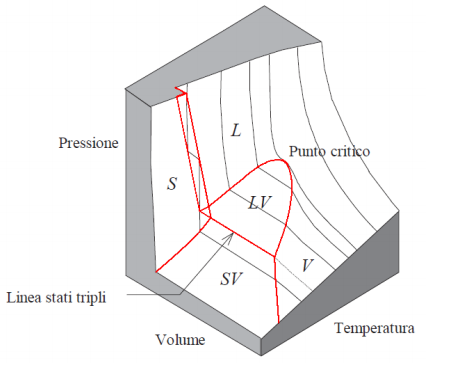
\includegraphics[height=5cm]{../L01/img4.PNG}
\end{center}
Lo stato termodinamico (punto appartenente alla superficie di stato) può anche essere geometricamente
rappresentato da un punto su un piano cartesiano sui cui assi vi sono due delle tre variabili prescelte.\newline
In particolare si possono realizzare piani termodinamici in coordinate (P,v), (P,T) e (T,v).
\subsubsection{Equazione di stato per i gas ideali}
\[
    PV=NRT
\]
$P$: pressione [$Pa$]\newline
$V$: volume [$m^3$]\newline
$N$: moli [$kmole$]\newline
$T$: temperatura [$K$]\newline
$R$: costante universale dei gas ideali $\rightarrow R = 8314 [J/(kmole \; K)]$\newline
Oppure:
\[
    PV = MR^*T
\]
$M$: massa [$kg$]\newline
$M_m$: massa molare [$kg/kmole$]\newline
$R^*$: costante caratteristica del gas considerato $\rightarrow R^* = \frac{R}{M_m}$
\begin{center}
    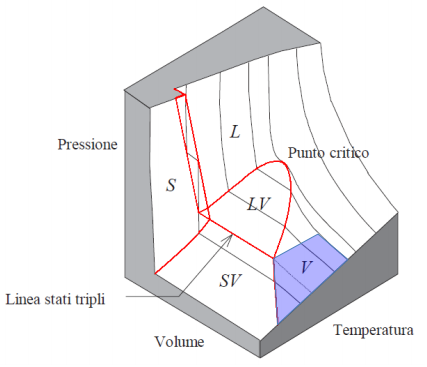
\includegraphics[height=5cm]{../L01/img5.PNG}
\end{center}
\subsubsection{Equazione di stato per i gas reali}
Modello di equazione di stato più complesso per descrivere il comportamento di gas in condizioni di \textbf{temperatura} e \textbf{pressioni elevate}.\newline
\newline
Equazione di van der Waals:
\[
    \left(P + \frac{a}{v_m^2}\right)(v_m - b) = RT
\]
Ove $a$ e $b$ sono caratteristiche del particolare gaas considerato:
\begin{center}
    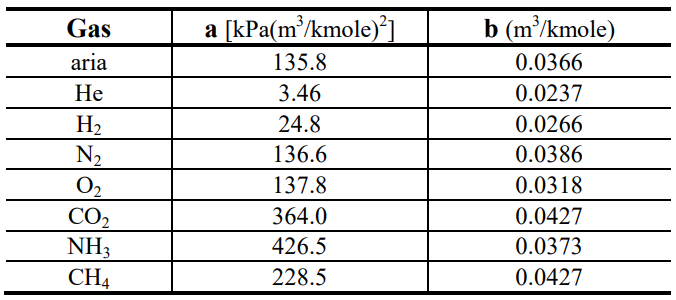
\includegraphics[height=3cm]{../L01/img8.PNG}
\end{center}
\begin{center}
    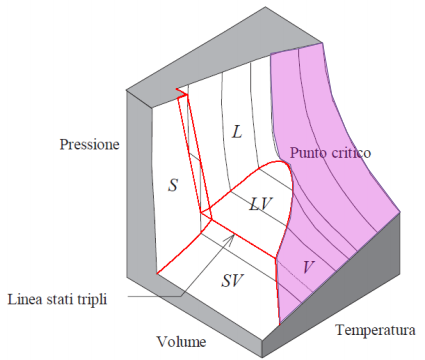
\includegraphics[height=5cm]{../L01/img6.PNG}
\end{center}
\subsubsection{Equazione di stato per liquidi e solidi}
\[
    dv = \beta v dT - K_T v dP
\]
\[
    \begin{matrix}
        \text{Coefficiente di dilatazioen termica isobaro}\; & \beta = \frac{1}{v}\left(\frac{\delta v}{\delta T}\right)_P\\
        \text{Coefficiente di comprimibilità isotermo}\; & K_T = - \frac{1}{v}\left( \frac{\delta v}{ \delta P} \right)_T
    \end{matrix}
\]
Siccome $\beta$ e $K_T$ possono essere considerati costanti per ampi intervalli di temperatura e di pressione, la precedente relazione differenziale è integrabile e lo stato calcolabile.
\begin{center}
    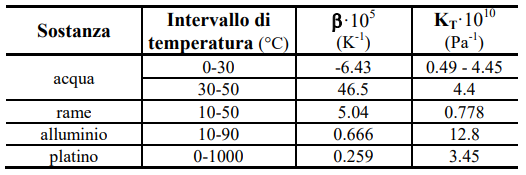
\includegraphics[height=3cm]{../L01/img9.PNG}
\end{center}
\begin{center}
    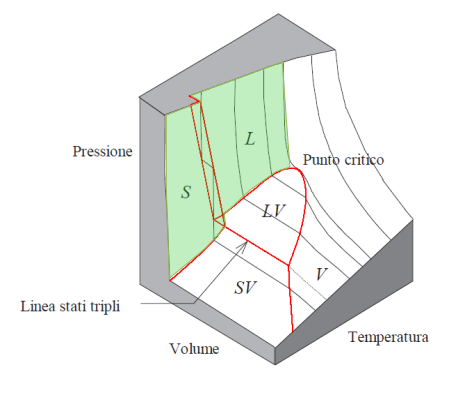
\includegraphics[height=5cm]{../L01/img7.PNG}
\end{center}
Un modello semplificato è quello per \textbf{liquidi e solidi incomprimibili}, in cui si considera $v =$ costante.